% !TeX encoding = UTF-8

\documentclass{protokol}

\usepackage{tikz}
\usetikzlibrary{calc}
\usetikzlibrary{arrows}

%====== Units =====
\usepackage{siunitx}
\sisetup{inter-unit-product =\ensuremath{\cdot}}
\sisetup{group-digits = integer}
\sisetup{output-decimal-marker = {,}}
\sisetup{exponent-product = \ensuremath{\cdot}}
\sisetup{separate-uncertainty}
\sisetup{tight-spacing = false}
%\sisetup{scientific-notation = true}
%\sisetup{round-mode=places,round-precision=4}
%\sisetup{evaluate-expression}


%====== Grafy =====
\usepackage{pgfplots}
\pgfplotsset{width=0.8\linewidth, compat=1.17}
\def\plotcscale{0.8}
\usepackage{pgfplotstable}
\usepackage[figurename=Obr.]{caption} % figure caption rename
%====== Rovnice align block ======
\usepackage{amsmath}
\setlength{\jot}{10pt} % rozestup mezi řádky

\graphicspath{ {./img/} }

%====== Vyplňte údaje ======
\jmeno{Jakub Charvot}
\kod{240844}
\rocnik{2.}
\obor{MET}
\skupina{MET/4}
\spolupracoval{Radek Kučera}

\merenodne{29.\,9.\,2022}
\odevzdanodne{13.\,10.\,2022}
\nazev{Pracovní bod a jeho pohyb}
\cislo{1} %měřené úlohy

\predmet{Analogové elektronické obvody}
\ustav{Ústav mikroelektroniky}
\skola{FEKT VUT v Brně}

\def\para{x+0}
\def\parb{\para-80}


\begin{document}
	%====== Vygenerování tabulky ======
	\maketitle
	%====== Úvodní texty protokolu ======
	
	\section{Teoretický úvod}
	
	\subsection{Bipolární tranzistor}
%	\subsubsection{Důležité parametry a vztahy}
		$ h_{21E}=\frac{I_{C Q}}{I_{B Q}} $~\dots~stejnosměrné proudové zesílení\\
		$ h_{21e}=\beta=\left.\frac{d I_C}{d I_B}\right|_Q $~\dots~střídavé proudové zesílení\\
		$ S=\left.\frac{d I_C}{d U_{B E}}\right|_Q $~\dots~strmost tranzistoru\\
		$ r_{i n}=\left.\frac{d U_{B E}}{d I_B}\right|_Q $~\dots~střídavý vstupní odpor\\
		$ r_{out}=\left.\frac{d U_{C E}}{d I_C}\right|_Q $~\dots~střídavý výstupní odpor\\
		\begin{figure}[h!]
			\centering
			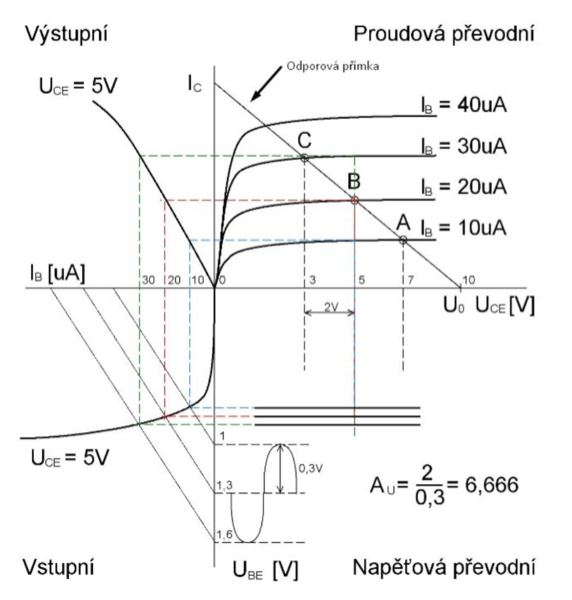
\includegraphics[width=0.6\textwidth]{bipolar.png}
			\centering
			\caption{Charakteristika bipolárního tranzistoru a pohyb pracovního bodu.}
			\label{fig:bipolar}
		\end{figure}\\
	
		
	\subsection{Unipolární tranzistor}
%	\subsubsection{Důležité parametry a vztahy}
		$ G_m=\frac{I_{D Q}}{U_{G S Q}} $~\dots~stejnosměrná strmost\\
		$ g_m=\left.\frac{d I_D}{d U_{G S}}\right|_Q $~\dots~střídavá strmost\\
		$ R_{i n}=\frac{R_{g_1} R_{g_2}}{R_{g_1}+R_{g 2}} $~\dots~střídavý vstupní odpor
		\begin{figure}[h!]
			\centering
			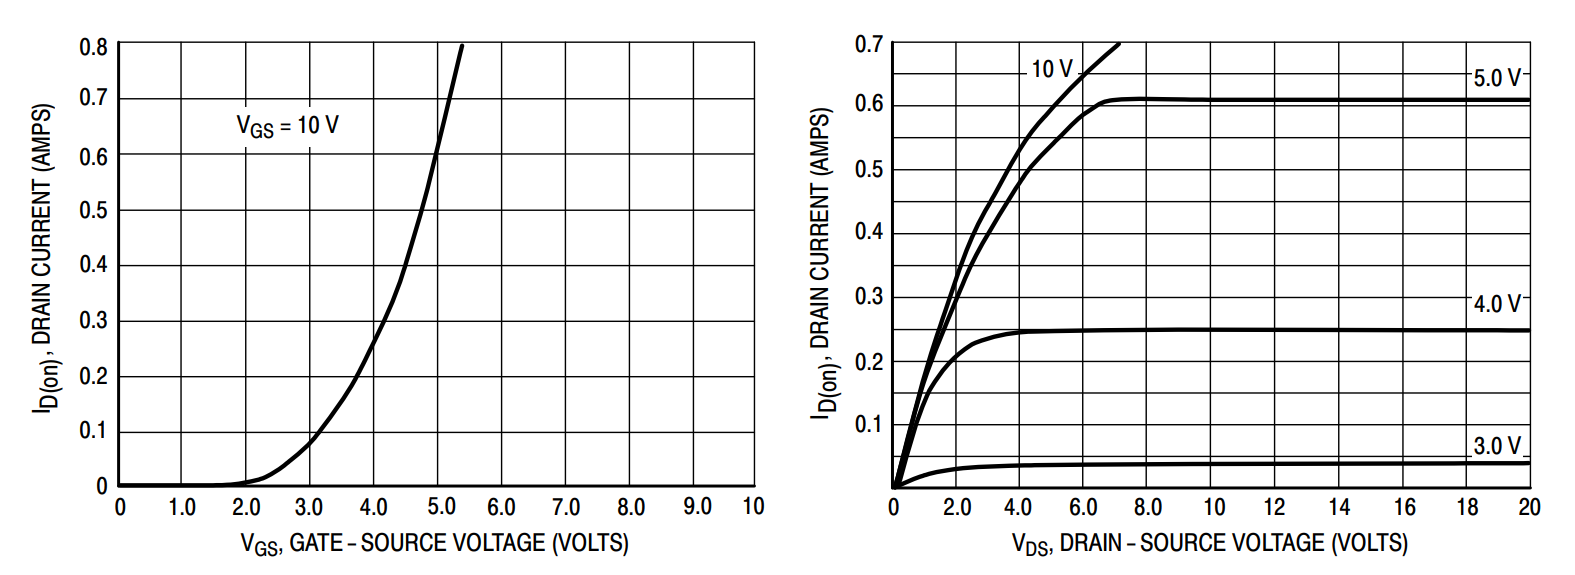
\includegraphics[width=\textwidth]{bs107a.png}
			\centering
			\caption{Převodní a výstupní charakteristika tranzistoru MOSFET (BS107A).}
			\label{fig:bs107a}
		\end{figure}\\
	
	
	
	\section{Zadání úlohy}
	\begin{figure}[h!]
		\centering
		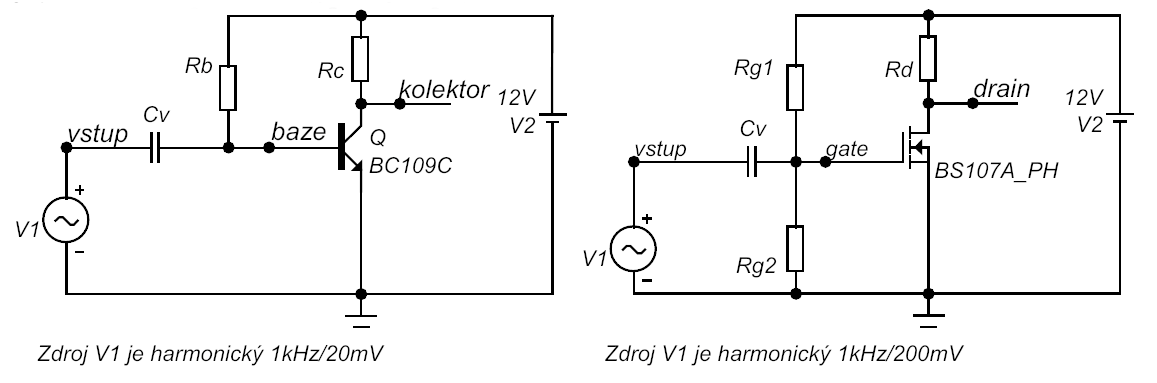
\includegraphics[width=\textwidth]{schemata.png}
		\centering
		\caption{Schémata zapojení obou úloh.}
		\label{fig:bs107a}
	\end{figure}
		V případě naší úlohy používáme bipolární tranzistor BC109C typu NPN a unipolární tranzistor BS107A typu MOSFET. Vycházíme z těchto zadaných parametrů:
		
	\subsubsection{BC109C}
	$ h_{21e}=\beta\approx h_{21E}\approx 500, S=0,1~A\cdot V^{-1}, r_{in}\approx 5~k\Omega, r_{out}\approx 100~k\Omega$
	
	\subsubsection{BS107A}
	$ G_{m}\approx 2~mA\cdot V^{-1}, g_{m}\approx6~mA\cdot V^{-1}$
	
	\subsection{Výsledky z numerického cvičení}
		\subsubsection{Zesilovač s bipolárním tranzistorem}
		$ R_{C}=2,2~k\Omega, R_{B}=2~M\Omega, C_V=5~\mu F $
		
		\noindent Stejnosměrný pracovní bod:\\
		$ U_{CE}\approx 6~V, I_{C}\approx2,73~mA, U_{BE}\approx0,65~V, I_{B}\approx5,46~\mu A$
		
		\noindent Střídavé poměry v obvodu:\\
		$ \dot{U}_{B E}=20~mV, \dot{I}_B=4~\mu A, \dot{U}_{out}=-4,4~V, \dot{I}_C=2~mA, f_{0}=6,4~Hz $
	
		\subsubsection{Zesilovač s unipolárním tranzistorem}
		$ R_{d}=2,2~k\Omega, R_{g1}=7,8~M\Omega, R_{g2}=1~M\Omega, C_V=10~nF $
		
		\noindent Stejnosměrný pracovní bod:\\
		$ U_{DS}\approx 6~V, I_{C}\approx2,73~mA, U_{GS}\approx1,365~V, I_{G}\approx0~A$
		
		\noindent Střídavé poměry v obvodu:\\
	$ \dot{U}_{GS}=200~mV, \dot{I}_G=0~A, \dot{U}_{out}=-2,64~V, \dot{I}_D=1,2~mA, f_{0}=18~Hz $
	
	\newpage
\section{Výsledky počítačové simulace}
\subsection{Bipolární tranzistor}

	\begin{figure}[h!]
		\centering
		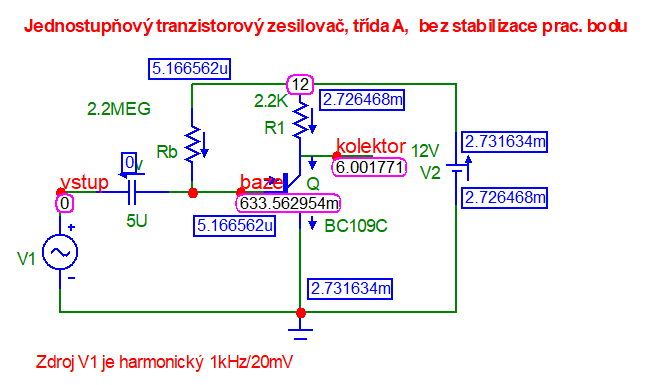
\includegraphics[width=\textwidth]{microcap/BJT/1_Pracovni_bod_zesilovace.png}
		\centering
		\caption{Pracovní bod zesilovače s BT.}
		\label{fig:mc_bt_prac_bod}
	\end{figure}

	\begin{figure}[h!]
		\centering
		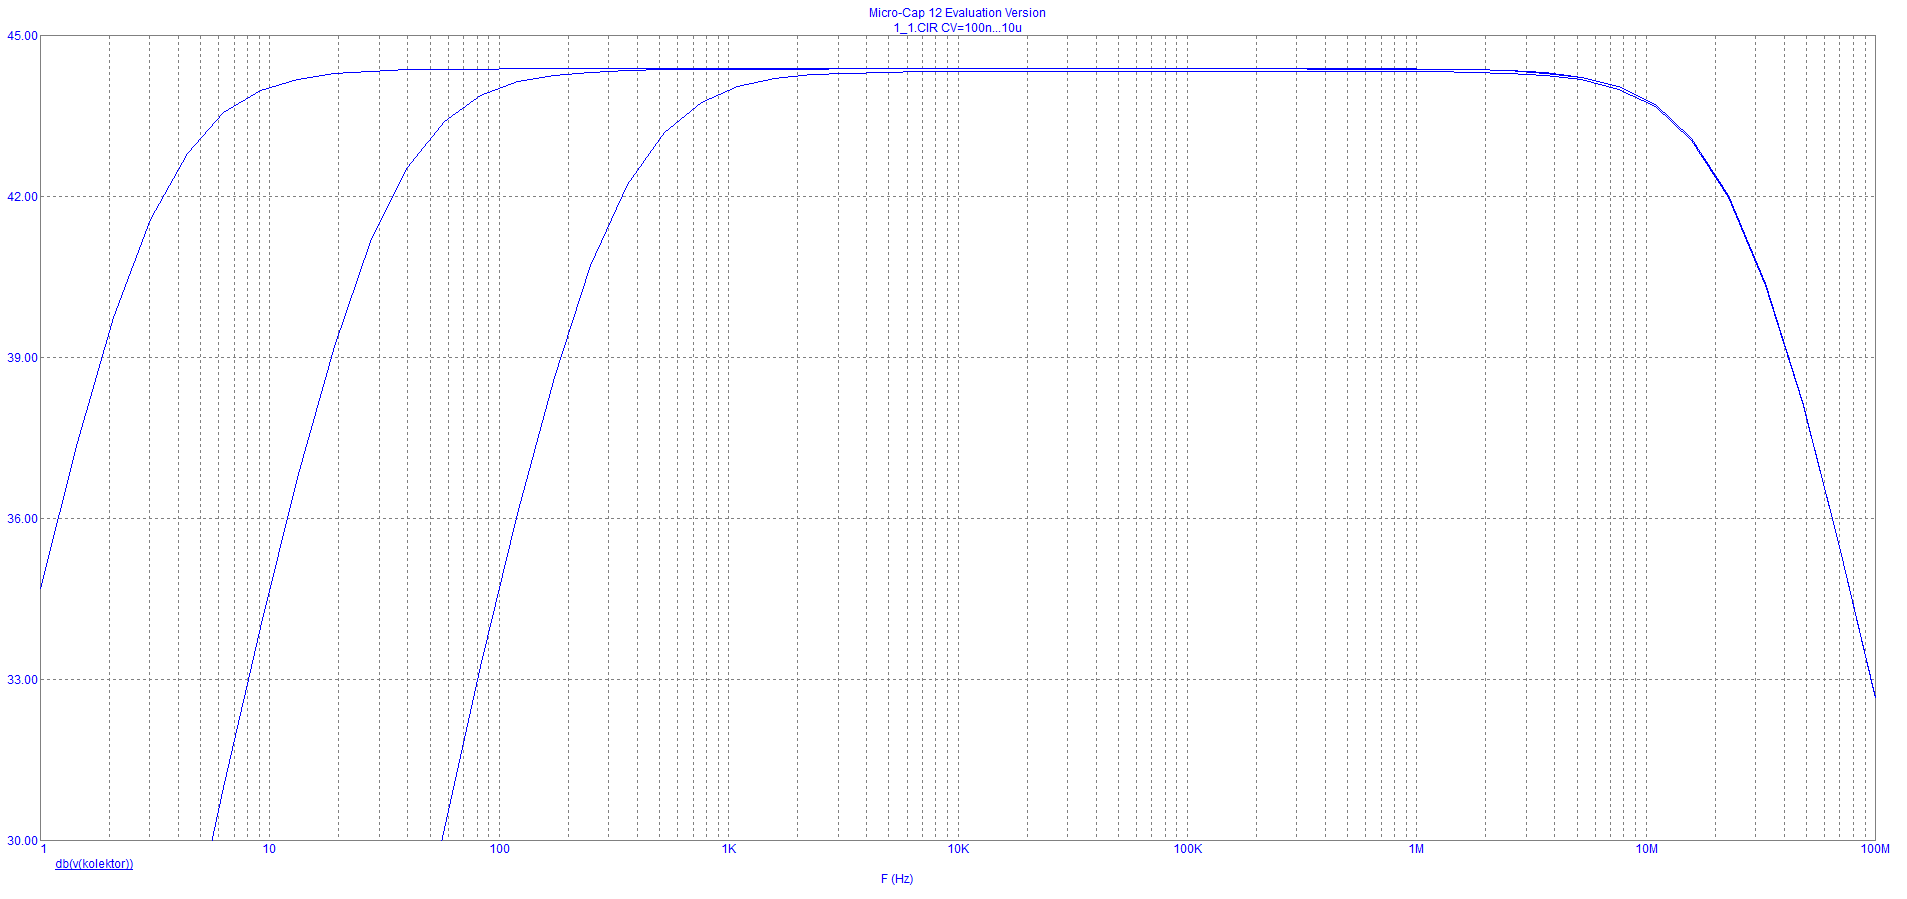
\includegraphics[width=\textwidth]{microcap/BJT/Frekvecni_prubeh_Cv_step.png}
		\centering
		\caption{Kmitočtová charakteristika zesilovače s BT, $ C_V= \{\SI{100}{\nano\farad};\SI{4.7}{\micro\farad};\SI{10}{\micro\farad}\} $.}
		\label{fig:-mc_}
	\end{figure}
	
	\begin{figure}[h!]
		\centering
		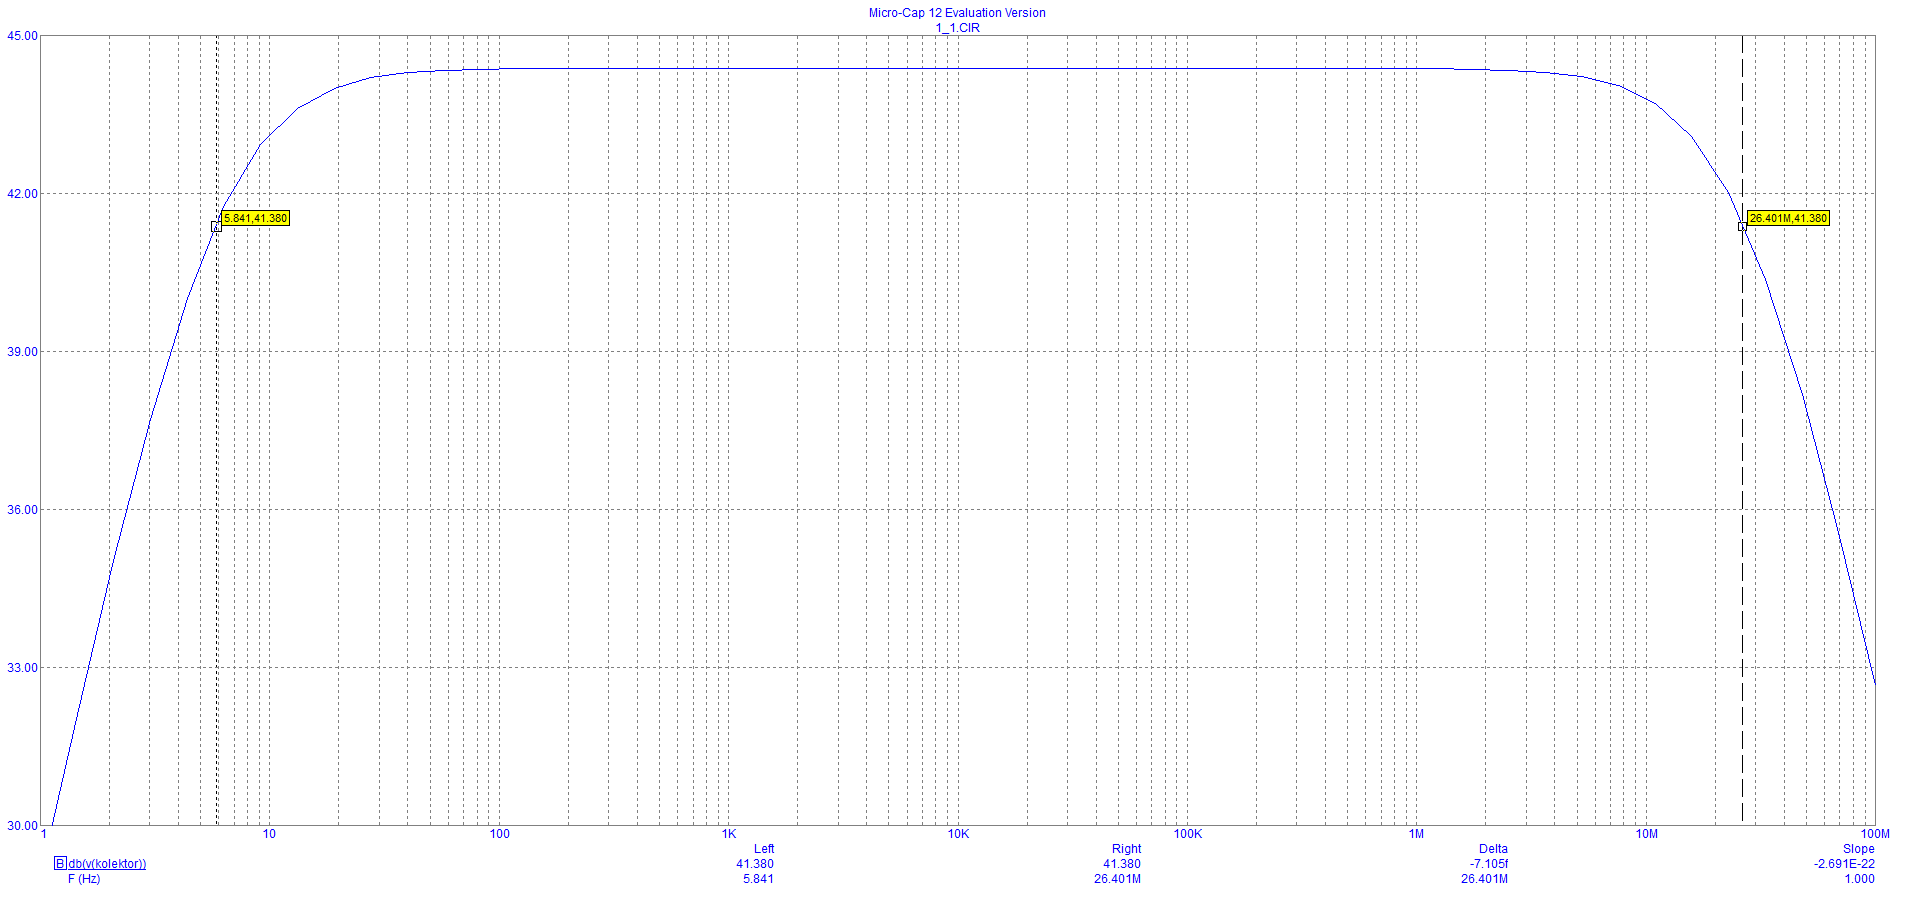
\includegraphics[width=\textwidth]{microcap/BJT/Frekvecni_prubeh.png}
		\centering
		\caption{Šířka pásma zesilovače s BT.}
		\label{fig:-mc_}
	\end{figure}
	
	\begin{figure}[h!]
		\centering
		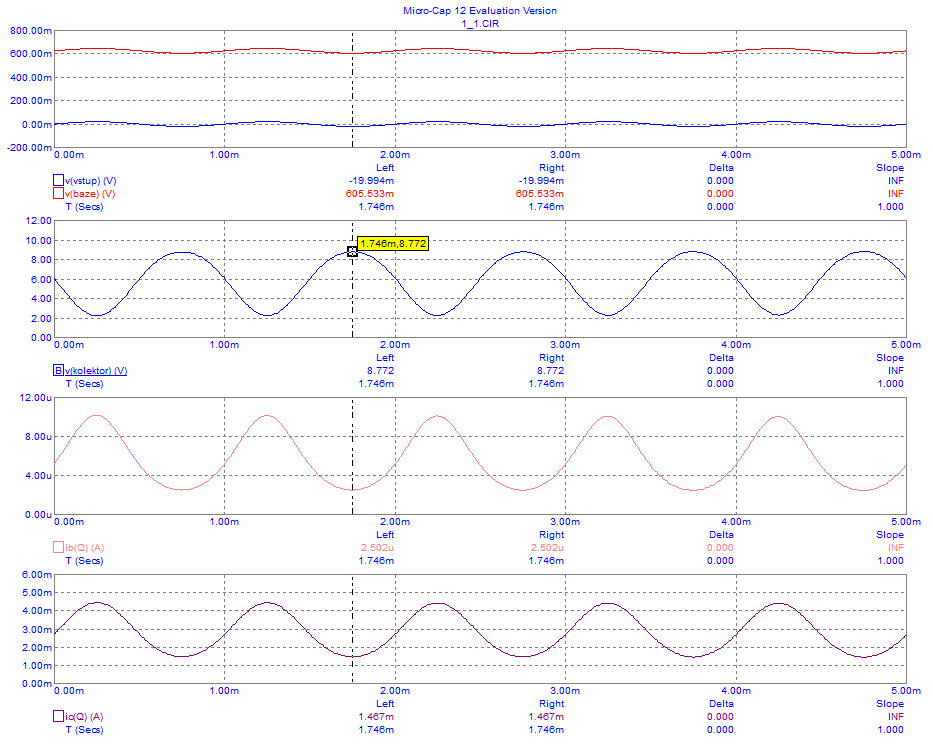
\includegraphics[width=\textwidth]{microcap/BJT/Prubehy_1.png}
		\centering
		\caption{Průběhy napětí a proudů pro zesilovač s BT.}
		\label{fig:-mc_}
	\end{figure}
	
	\begin{figure}[h!]
		\centering
		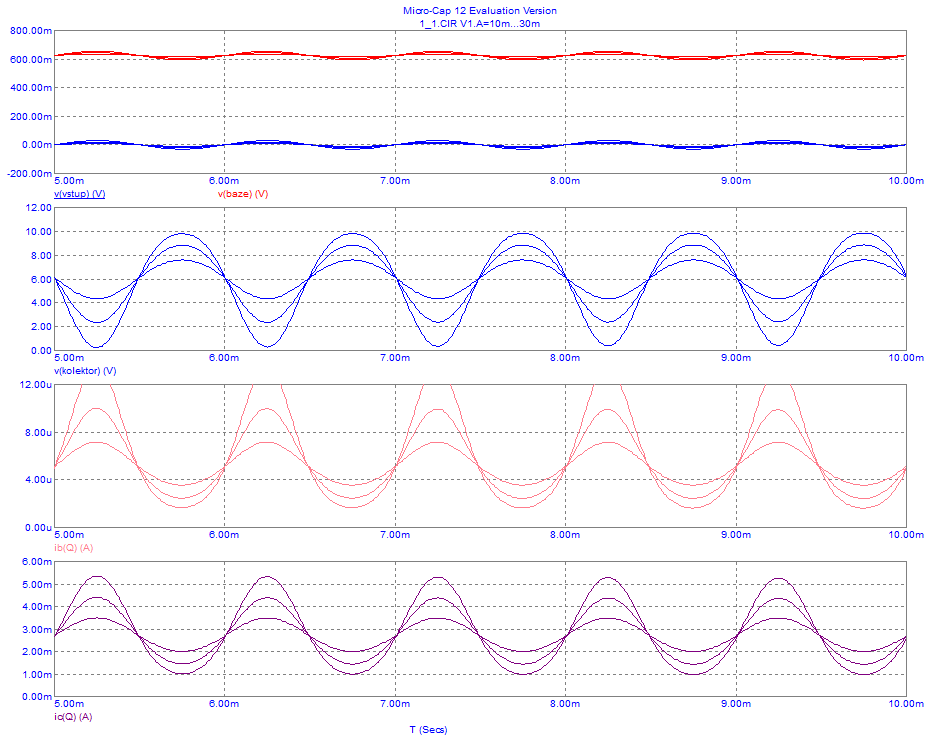
\includegraphics[width=\textwidth]{microcap/BJT/Prubehy_2_10mV-30mV.png}
		\centering
		\caption{Reakce obvodu na změnu amplitudy vstupního signálu, $ U_{in}= \{\SI{10}{\milli\volt};\SI{20}{\milli\volt};\SI{30}{\milli\volt}\} $.}
		\label{fig:-mc_}
	\end{figure}
	
	\begin{figure}[h!]
		\centering
		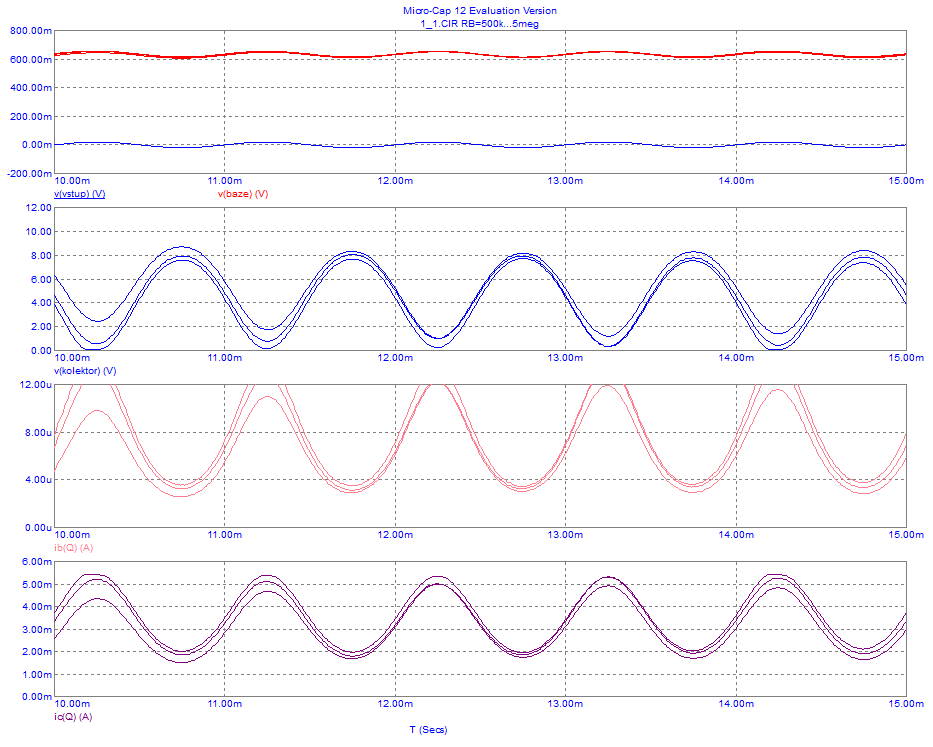
\includegraphics[width=\textwidth]{microcap/BJT/Prubehy_2_RB_500k-5M.png}
		\centering
		\caption{Změna pracovního bodu tranzistoru, $ R_{b}= \{\SI{0.5}{\mega\ohm};\SI{2}{\mega\ohm};\SI{5}{\mega\ohm}\} $.}
		\label{fig:-mc_}
	\end{figure}

\clearpage
\subsection{Unipolární tranzistor}	
	\begin{figure}[h!]
		\centering
		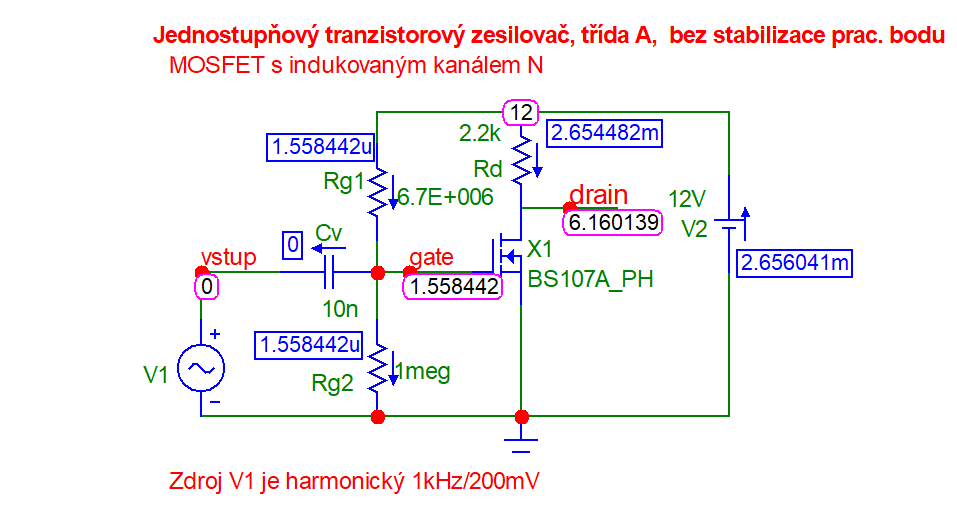
\includegraphics[width=\textwidth]{microcap/xFET/1_Pracovni_bod_zesilovace.png}
		\centering
		\caption{Pracovní bod zesilovače s unipolárním tranzistorem.}
		\label{fig:mc_ut_prac_bod}
	\end{figure}
	
	\begin{figure}[h!]
		\centering
		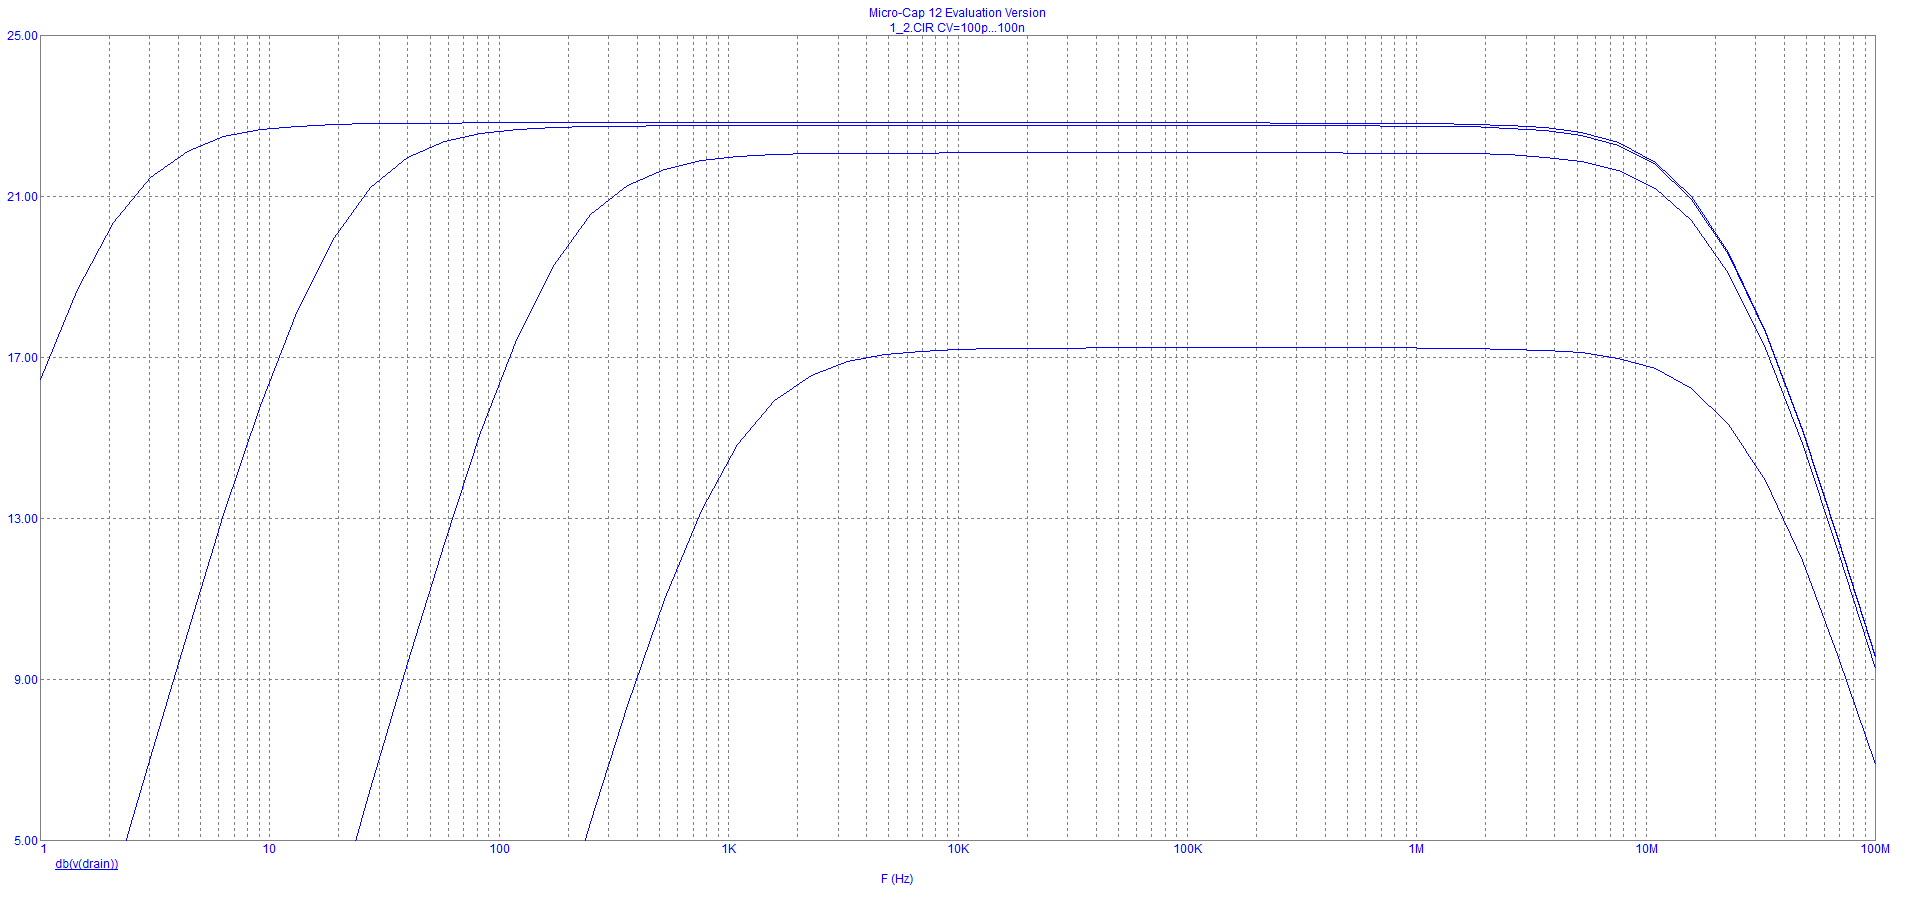
\includegraphics[width=\textwidth]{microcap/xFET/Frekvecni_prubeh_Cv_step.png}
		\centering
		\caption{Kmitočtová charakteristika zesilovače s UT, $ C_{V}= \{\SI{100}{\pico\farad};\SI{1}{\nano\farad};\SI{10}{\nano\farad};\SI{100}{\nano\farad}\} $.}
		\label{fig:-mc_}
	\end{figure}
	
	\begin{figure}[h!]
		\centering
		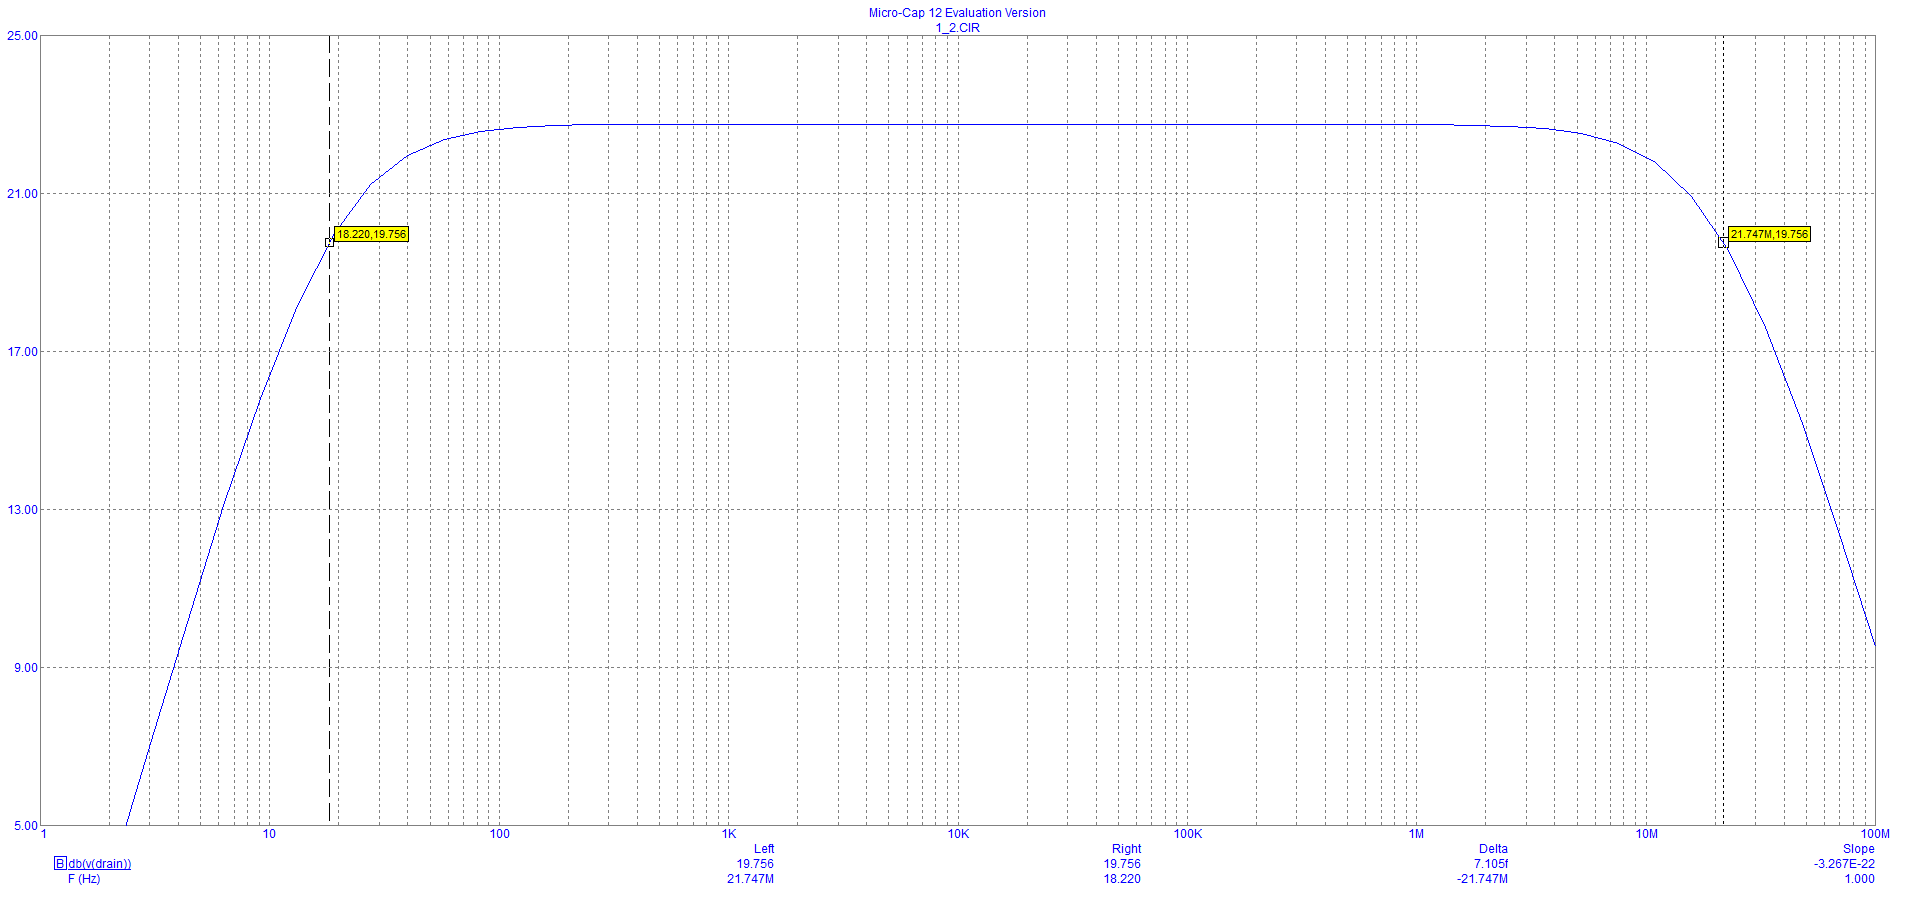
\includegraphics[width=\textwidth]{microcap/xFET/Frekvecni_prubeh.png}
		\centering
		\caption{Šířka pásma zesilovače s UT.}
		\label{fig:-mc_}
	\end{figure}
	
	\begin{figure}[h!]
		\centering
		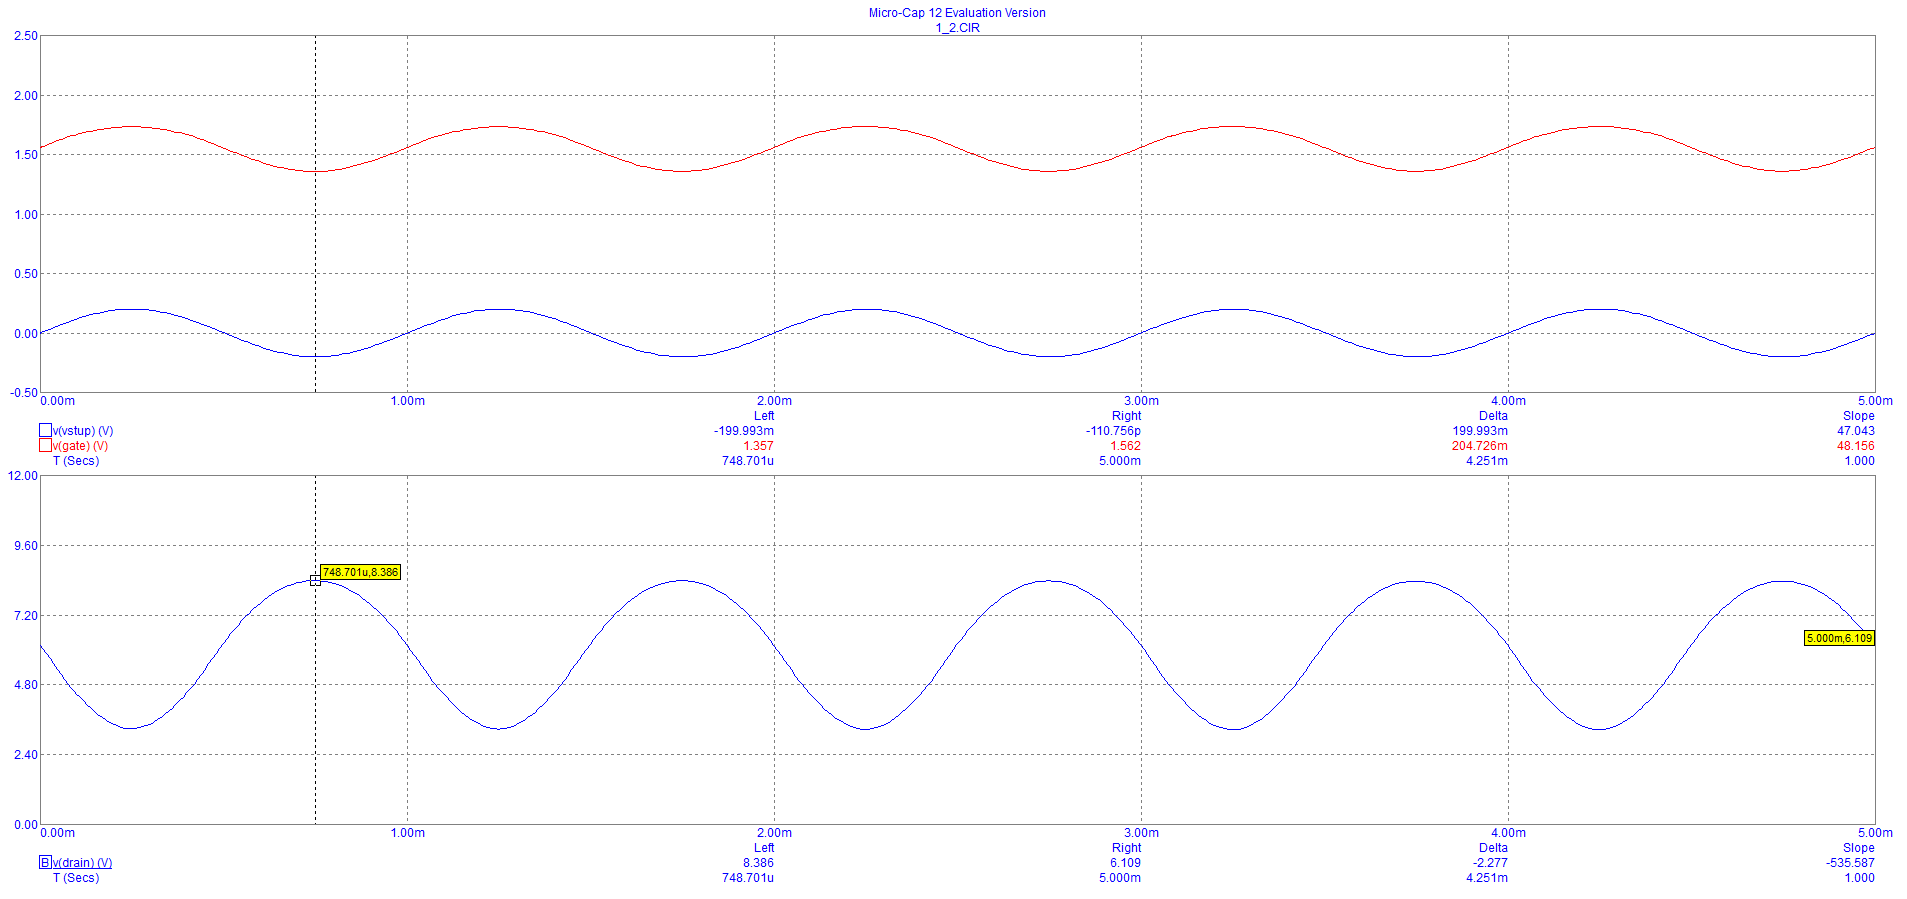
\includegraphics[width=\textwidth]{microcap/xFET/Prubehy_1.png}
		\centering
		\caption{Časová závislost napětí v obvodu.}
		\label{fig:-mc_}
	\end{figure}
	
	\begin{figure}[h!]
		\centering
		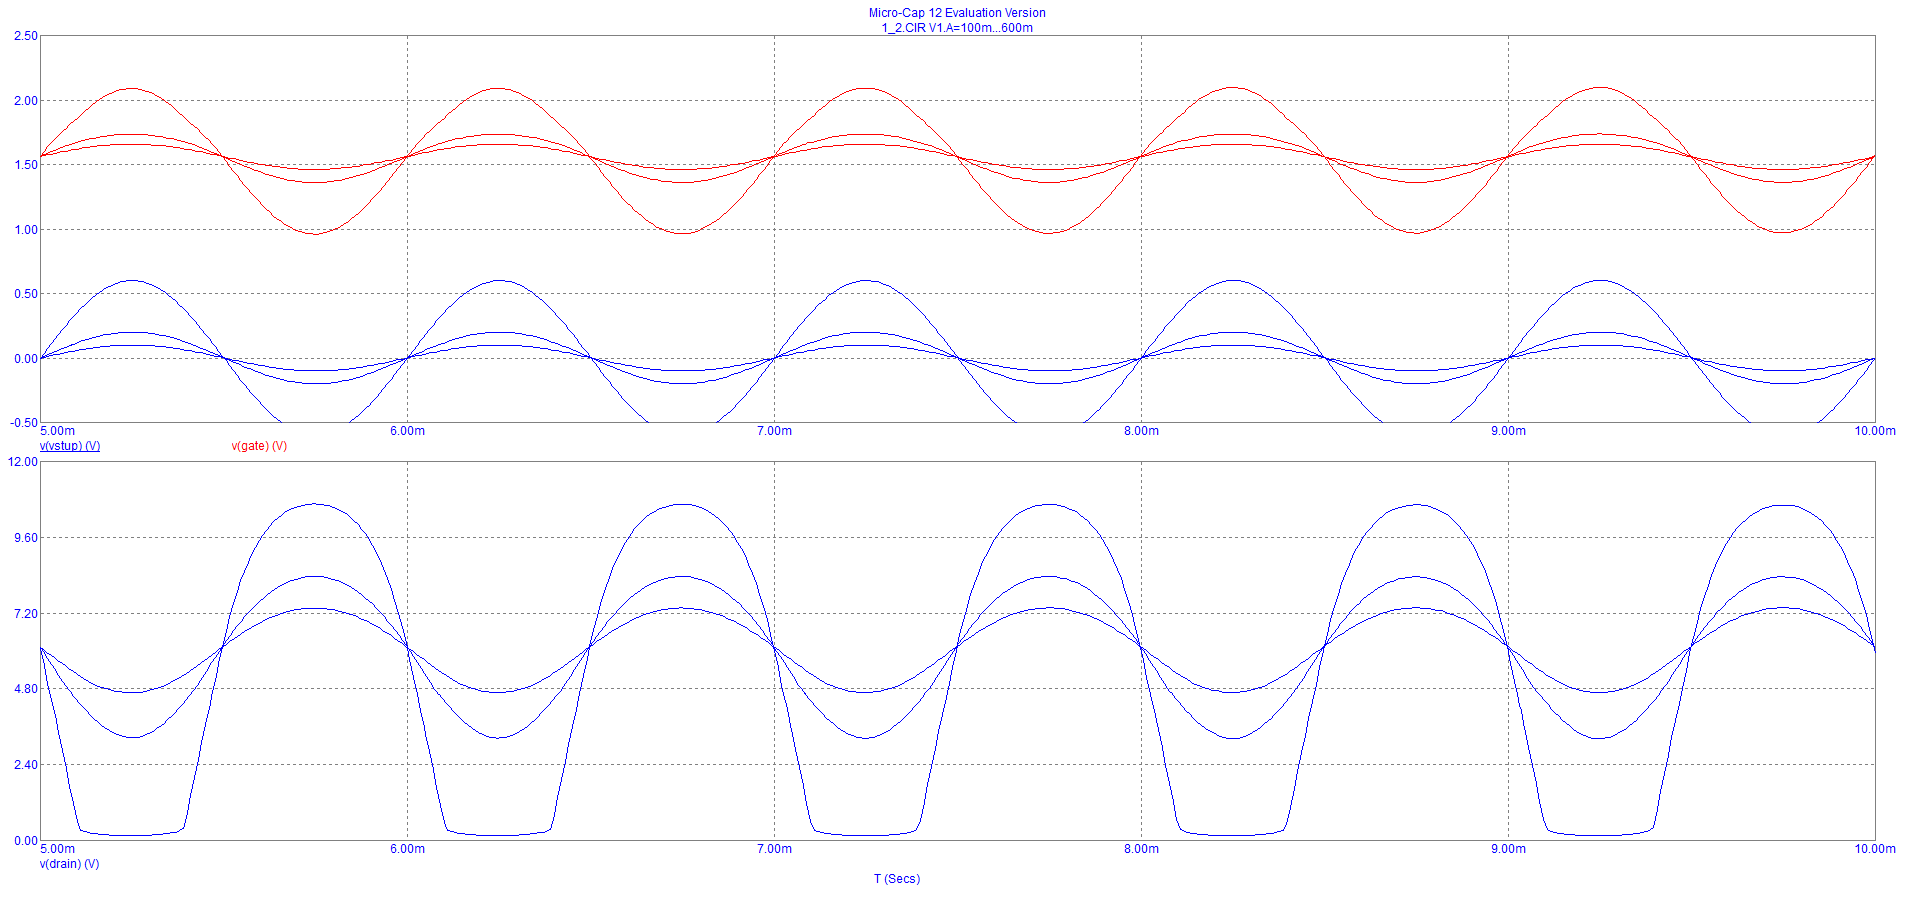
\includegraphics[width=\textwidth]{microcap/xFET/Prubehy_2_100mV-600mV.png}
		\centering
		\caption{Reakce obvodu s UT na změnu amplitudy vstupního napětí,  $ U_{in}= \{\SI{100}{\milli\volt};\SI{200}{\milli\volt};\SI{600}{\milli\volt}\} $.}
		\label{fig:-mc_}
	\end{figure}
	
	\begin{figure}[h!]
		\centering
		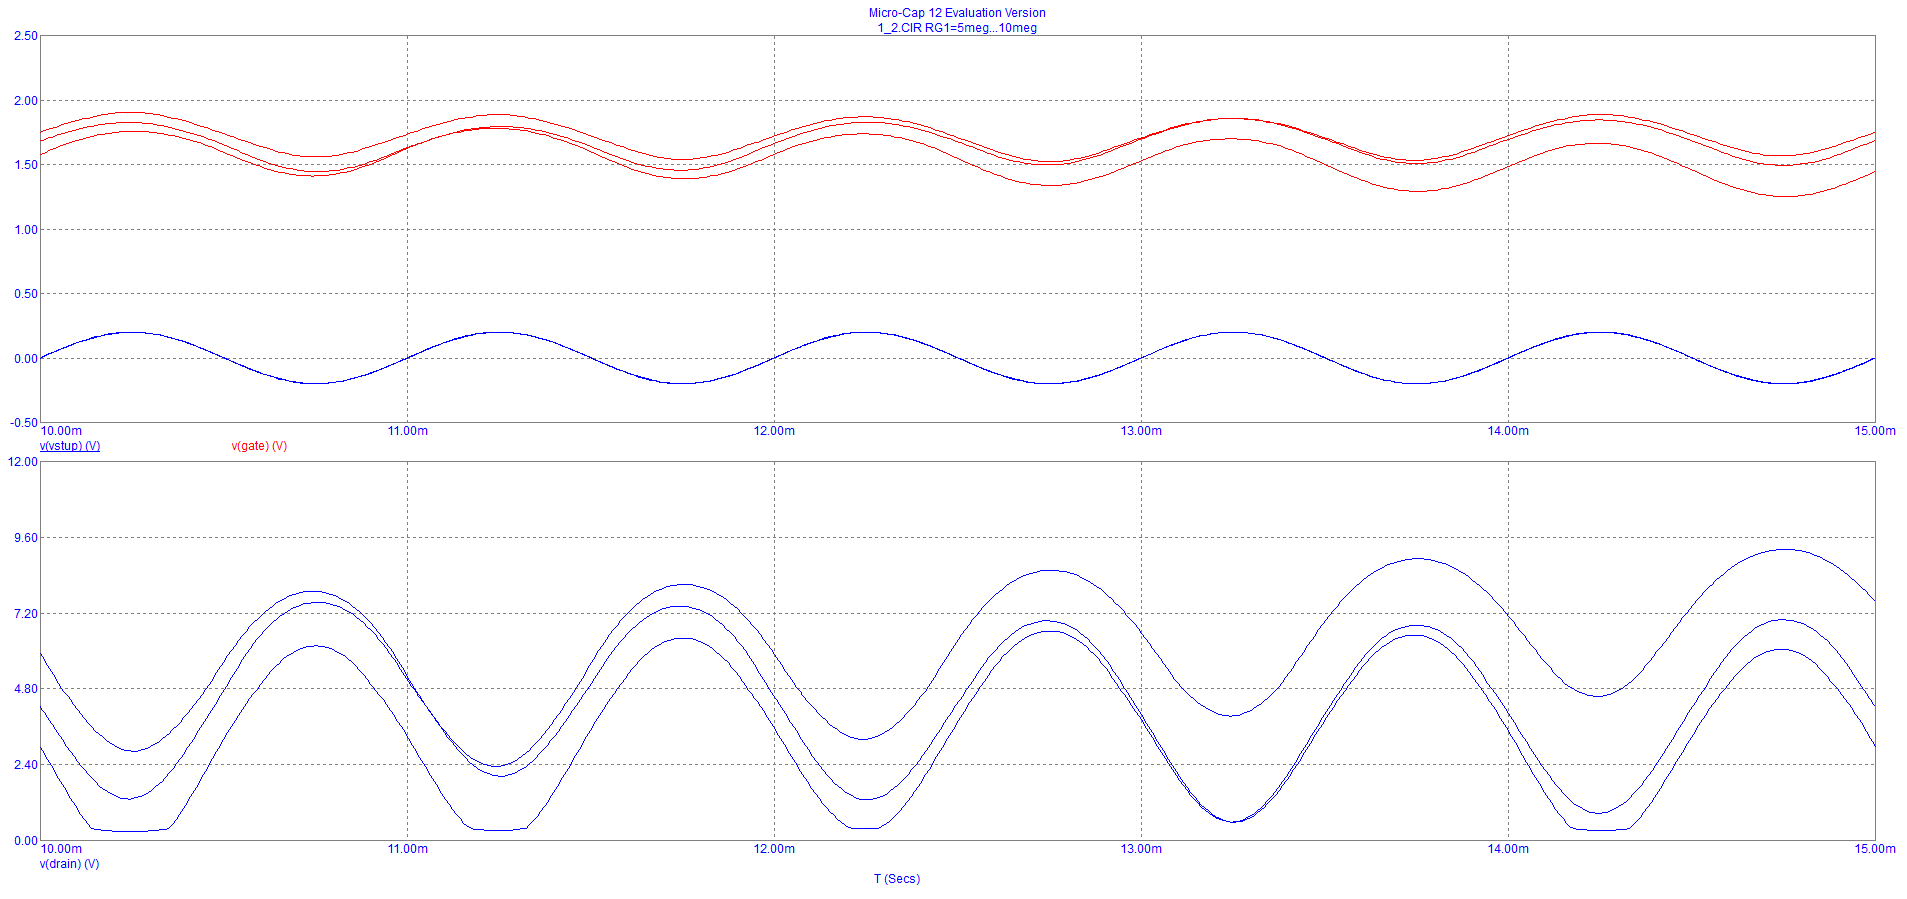
\includegraphics[width=\textwidth]{microcap/xFET/Prubehy_2_RB_5M-10M.png}
		\centering
		\caption{Změna pracovního bodu tranzistoru, $ R_{b}= \{\SI{5}{\mega\ohm};\SI{6.7}{\mega\ohm};\SI{10}{\mega\ohm}\} $.}
		\label{fig:-mc_}
	\end{figure}
	
	
	\begin{figure}[h!]
		\centering
		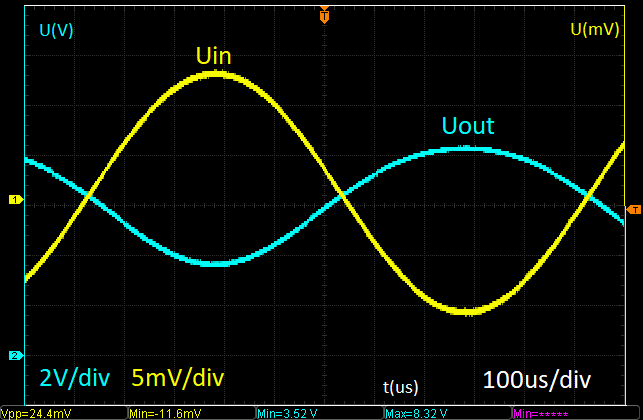
\includegraphics[width=\textwidth]{oscilo/1done.png}
		\centering
		\caption{Nezkreslené zesílení.}
		\label{fig:-osc_}
	\end{figure}
	
	\begin{figure}[h!]
		\centering
		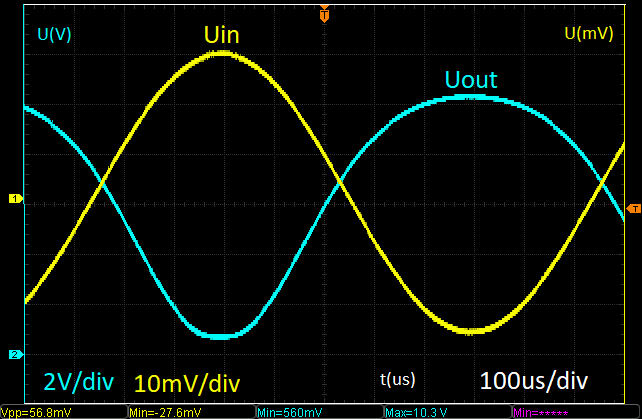
\includegraphics[width=\textwidth]{oscilo/2done.png}
		\centering
		\caption{Mírné zkreslení, vyšší amplituda vstupního signálu.}
		\label{fig:-osc_}
	\end{figure}
	
	\begin{figure}[h!]
		\centering
		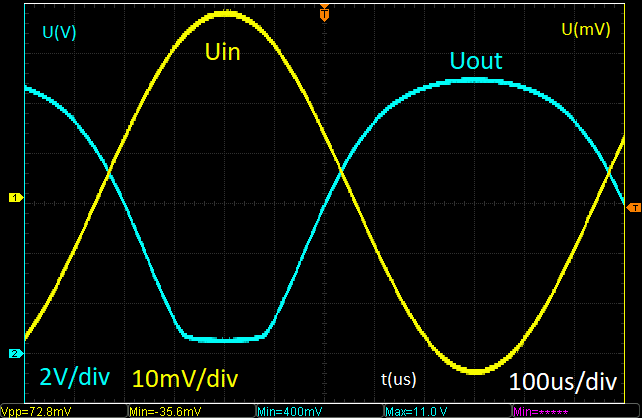
\includegraphics[width=\textwidth]{oscilo/3done.png}
		\centering
		\caption{Vysoké zkreslení, dosažení saturace.}
		\label{fig:-osc_}
	\end{figure}
	
	\begin{figure}[h!]
		\centering
		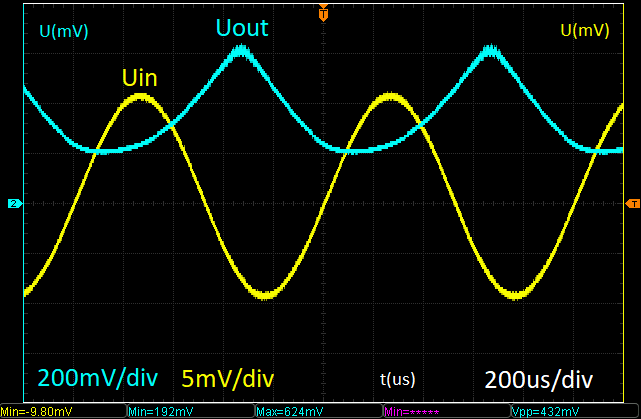
\includegraphics[width=\textwidth]{oscilo/4done.png}
		\centering
		\caption{Změna pracovního bodu,$ R_b=\SI{1}{\mega\ohm} $.}
		\label{fig:-osc_}
	\end{figure}
	
	\begin{figure}[h!]
		\centering
		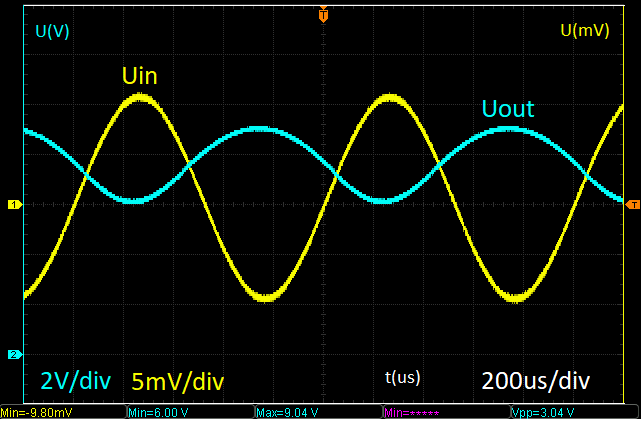
\includegraphics[width=\textwidth]{oscilo/5done.png}
		\centering
		\caption{Změna pracovního bodu,$ R_b=\SI{4,16}{\mega\ohm} $.}
		\label{fig:-osc_}
	\end{figure}

	\begin{figure*}[h!]
		\begin{tikzpicture}
			\centering
			\begin{axis}
				[
				xlabel={$f\ [\unit{\hertz}]$},
				ylabel={$A_U\ [\unit{\deci\bel}]$},
				width=1\textwidth,
				height = 0.5\textwidth,
%				legend pos=south east,
				legend style={at={(0.99,0.025)},anchor=south east},
				xmode=log,
				xmin=0.1,
				xmax=1e7
				]
				% 4.7 muF
				\addplot[mark=x, blue, smooth, mark size=3pt] table [skip first n=2, x=f47, y=A47, col sep=comma] {data/data.csv};
				\addlegendentry{\SI{4.7}{\micro\farad}}
				% 10 muF
				\addplot[mark=x, red, smooth, mark size=3pt] table [skip first n=2, x=f10, y=A10, col sep=comma] {data/data.csv};
				\addlegendentry{\SI{10}{\micro\farad}}
				% 100 nF
				\addplot[mark=x, green, smooth, mark size=3pt] table [skip first n=2, x=f100, y=A100, col sep=comma] {data/data.csv};
				\addlegendentry{\SI{100}{\nano\farad}}
				% -3dB
				\addplot [
				domain=0.1:1e7, 
				samples=2, 
				color=gray,
				dashed,
				no marks
				]
				{43.18};		
				
				% Proměnné pro popisky a vynášecí čáry
				\def\firstx{3}
				\def\secondx{5.5}
				\def\thirdx{235}
				\def\fourthx{4.5e5}
				\def\topy{44.3}
				\def\bottomy{3}
				\def\labeltop{12}
				
				\node[] (A) at (axis cs: \firstx,\bottomy) {};
				\node[] (Alabel) at (axis cs: \firstx,\labeltop) {};
				\node[] (AA) at (axis cs: \firstx,\topy) {};
				\node[] (B) at (axis cs: \secondx,\bottomy) {};
				\node[] (Blabel) at (axis cs: \secondx,\labeltop) {};
				\node[] (BB) at (axis cs: \secondx,\topy) {};
				\node[] (C) at (axis cs: \thirdx,\bottomy) {};
				\node[] (Clabel) at (axis cs: \thirdx,\labeltop) {};
				\node[] (CC) at (axis cs: \thirdx,\topy) {};
				\node[] (D) at (axis cs: \fourthx,\bottomy) {};
				\node[] (Dlabel) at (axis cs: \fourthx,\labeltop) {};
				\node[] (DD) at (axis cs: \fourthx,\topy) {};
				\node[] (Elabel) at (axis cs: 0.1,47.5) {};

			\end{axis}    
		
		\node[anchor=north east] (label) at (Alabel) {\SI{3}{\hertz}};
		\node[anchor=north west] (label) at (Blabel) {\SI{5.5}{\hertz}};
		\node[anchor=north west] (label) at (Clabel) {\SI{235}{\hertz}};
		\node[anchor=north east] (label) at (Dlabel) {\SI{4.5e5}{\hertz}};
		\node[anchor=north west] (label) at (Elabel) {\SI{43,18}{\deci\bel}};
		\draw (A) -- (AA);
		\draw (B) -- (BB);
		\draw (C) -- (CC);
		\draw (D) -- (DD);
		
		\end{tikzpicture}
		\caption{Kmitočtová charakteristika zesilovače v závislosti na změně hodnoty vazebního kapacitoru $ C_V $.}
		\label{fig:graf_fajny}
	\end{figure*}


\clearpage
\section{Tabulka hodnot}
\begin{table}[h!]
	\centering
	\def\arraystretch{1.4}
	\centering
	\begin{tabular}{|c|c|c|c|c|}	
		\hline
		& $U_{CE} \; [V]$ & $U_{CB} \; [V]$ & $U_{BE}\; [mV]$ & $h_{21E} \; [-]$ \\ [0.1ex]
		\hline
		Výpočet   &6,000  &11,350 &650,000&500\\ [0.1ex]
		\hline 
		Simulace  &6,001 &11,366 &633,563&520  \\[0.1ex]
		\hline
		Měření    &6,000 & - & - &570\\[0.1ex]
		\hline
	\end{tabular}
		\caption{Porovnání výsledků.}
		\label{tab:porovnani}
\end{table}


\section{Závěr}
	Stanovovali jsme pracovní bod zapojení s bipolárním a unipolárním tranzistorem a určovali jejich kmitočtové charakteristiky. Hodnoty vypočtené v numerických a počítačových cvičeních se liší minimálně, na základě takto zjištěných hodnot jednotlivých součástek je možné realizovat praktické zapojení. Jelikož ale činitel $ h_{21E} $ velmi závisí na konkrétním kusu tranzistoru a v našel případě je o něco vyšší než bylo předpokládáno (viz. Tab.~\ref{tab:porovnani}), bylo potřeba upravit hodnotu odporu $ R_B $ na \SI{3,02}{\mega\ohm}.
	
	Na základě simulace jsme testovali zkreslení signálu jak při zvýšení amplitudy vstupního signálu, tak při změně pracovního bodu (změna hodnoty $ R_b $). Pro příliš velkou amplitudu vstupního signálu se tranzistor dostává mimo oblast lineárního zesílení, do oblasti saturace, dochází tedy ke zkreslení signálu. Stejně tak tomu je i v případě snížení hodnoty $ R_b $. Při zvýšení hodnoty $ R_b $ tranzistor méně zesiluje.
	
	Pro tři hodnoty vazebného kondenzátoru $ C_V $ jsme za pomocí osciloskopu měřili kmitočtovou charakteristiku zapojení (viz. Obr.~\ref{fig:graf_fajny}). Pro $ C_V=\SI{4.7}{\milli\farad} $ jsme stanovili dolní mezní kmitočet \SI{5.5}{\hertz}, což téměř odpovídá hodnodě určené simulací. Horní mezní kmitočet se už ale liší, naměřili jsme hodnotu \SI{0.45}{\mega\hertz}, naopak simulace zobrazila \SI{26.4}{\mega\hertz}.

\end{document} 
